%&../.preamble
\endofdump

\usetikzlibrary{external}
\tikzset{external/system call={pdflatex --shell-escape --fmt=../.preamble --halt-on-error -jobname "\image" "\endofdump\texsource"}}
\tikzexternalize[prefix=tikz/]

\title{Logica computazionale}
\author{Marini Mattia}
\date{$ 1^o $ semestre $ 3^o $ anno}

\begin{document}
\maketitle
\tableofcontents
\listofdefs
\newpage

\section{Mondo e mente}
\begin{definizione}{Fallacia}
	Una fallacia è un ragionamento logico invalido. Si distinguono in:
	\begin{enumerate}
		\item Fallace formali: l'errore sta nella struttura logica del ragionamento in se (es. paradossi)
		\item Fallace informali: errore "umano", non intrinseco al ragionamento (es. bias cognitivo, misconcezioni, over-generalizzazione, catastrofismo)
	\end{enumerate}
\end{definizione}
\begin{definizione}{Rappresentazione mentale}
	Parte della memoria di una persona che rappresenta il mondo giunto ad essa tramite i sensi
	\vskip3mm
	Può essere
	\begin{enumerate}
		\item Analogica: quanto ci giunge tramite i sensi
		\item Linguistica: descrizione linguistica della rapp analogica
	\end{enumerate}
\end{definizione}
\subsubsection*{Rappresentazioni mentali, analogiche, linguistiche}
\begin{definizione}{Gap semantico}
	Differenza fra il mondo effettivo e ciò che viene percepito di questo.
	\[
		\text{ world} \neq \text{world mental representation }
	\]
\end{definizione}
\begin{definizione}{Consistenza e inconsistenza rappresentazioni}
	Due rappresentazioni sono inconsistenti se è impossibile che rappresentino entrambe la stessa parte di mondo.
\end{definizione}
Es. una rappresenta una macchina gialla e l'altra la medesima macchina verde

\subsubsection*{Rappresentazione vs rappresentazione mentale}
Una rappresentazione mentale sta nella mente, mentre una rappresentazione è un qualcosa di fisico e tangibile:
\begin{center}
	\begin{tabular}{ l l l }
		\toprule
		            & Rapp. mentale     & Rappresenzatione                 \\
		\midrule
		Analogica   & ricordo paesaggio & dipinto paesaggio                \\
		Linguistica & manoscritto       & flusso parole nella nostra testa \\
		\bottomrule
	\end{tabular}
\end{center}
\subsection{Fatti e modelli}
\begin{definizione}{Fatto}
	Un fatto è qualcosa che accade a determinate \textit{coordinate} spazio temporali
\end{definizione}
\begin{definizione}{Modello}
	Un \textit{modello} è un insime di fatti
	\[
		M = \left\{f\right\}
	\]
	\textit{Nota:} Un fatto è una nozione primitiva e non può essere formalmente definita
\end{definizione}
Ad esempio i seguenti sono fatti:
\begin{enumerate}
	\item Sofia è una persona
	\item Sofia ha i capelli biondi
	\item Amo il gelato
\end{enumerate}
\begin{definizione}{Consistenza di un fatto}
	Due fatti sono inconsistenti se non possono coesistere in un modello del mondo come lo percepiamo
\end{definizione}
\begin{definizione}{Asserzione}
	Un'asserrzione $ a $ è una \underline{rappresentazione linguistica atomica di un fatto} $ f $.
	\vskip3mm
	Il modo più semplice è pensare ad un'asserzione come \textit{una relazione fra un soggetto e un oggetto}
\end{definizione}
ad esempio, \textit{Sofia è negra} è un'asserzione
\begin{definizione}{Teoria asserzionistica}
	Una teoria asserzionistica $ \mathcal{T}_{\mathcal{A}} $ è un insieme di asserzioni
	\[
		\mathcal{T}_{\mathcal{A}} = \left\{a\right\}
	\]
\end{definizione}
\begin{definizione}{Funzione di interpretazione di una teoria}
	Una funzione di interpretazione è una funzione:
	\[
		\mathcal{I}_{A} : \mathcal{T}_{\mathcal{A}} \rightarrow M
	\]
	che assegna ad un'asserzione $ a $ un fatto $ f $:
	\[
		\mathcal{I}_{A}\left(a\right) = f
	\]
\end{definizione}
\begin{definizione}{Polisemia (polysemy)}
	E' il fenomeno che crea ambiguità nei linguaggi naturali. Formalmente:
	\[
		\mathcal{I}_A\left(a\right) = f_1 \quad \text{ e } \quad \mathcal{I}_A\left(a\right) = f_2
	\]
\end{definizione}
\begin{definizione}{Sinonimia (synonymity)}
	E' il fenomeno per cui due parole hanno lo stesso significato. Formalmente:
	\[
		\mathcal{I}_A\left(a_1\right) = f \quad \text{ e } \quad \mathcal{I}_A\left(a_2\right) = f
	\]
\end{definizione}

\subsection{Dominio e linguaggio}
\begin{definizione}{Dominio}
	Un dominio è un insieme di fatti:
	\[
		F = \left\{f\right\}
	\]
	Il modello è un sottoinsieme del dominio:
	\[
		M \subseteq D
	\]
\end{definizione}
\begin{definizione}{Linguaggio asserzionistico}
	Un linguaggio asserzionistico è un insieme di asserzioni:
	\[
		\mathcal{L}_{A} = \left\{a\right\}
	\]
	La teoria è un sottoinsieme del linguaggio:
	\[
		\mathcal{T}_{\mathcal{A}} = \mathcal{L}_{A}
	\]
\end{definizione}
\begin{definizione}{Correttezza e completezza linguaggio}
	Un linguaggio $ \mathcal{L}_{A} $ è:
	\begin{enumerate}
		\item Completo se esiste un'asserzione per ogni elemento del dominio
		\item Corretto se non esistono asserzioni per elementi fuori dal dominio
	\end{enumerate}
\end{definizione}

\begin{definizione}{Funzione di interpretazione di un linguaggio}
	Una funzione di interpretazione è una funzione:
	\[
		\mathcal{I}_{A} : \mathcal{T}_{\mathcal{A}} \rightarrow M
	\]
	che assegna ad un'asserzione $ a $ un fatto $ f $:
	\[
		\mathcal{I}_{A}\left(a\right) = f
	\]
\end{definizione}

\subsection{Modelli di mondo}
\begin{definizione}{Modello di mondo}
	La coppia
	\[
		\mathcal{W} = \left<\mathcal{L}_{A}, D, \mathcal{I}_A\right>
	\]
	è detta \underline{modello di mondo}
\end{definizione}
Uno schema riassuntivo è il seguente:
\begin{center}
	\begin{tikzpicture}[node distance = 9em]
		\node (1)[] at (0,0) {$ a $};
		\node (2)[right of = 1] {$ \mathcal{T}a $};
		\node (3)[right of = 2] {$ \mathcal{L} a $};
		\node (4)[below of = 1] {$f$};
		\node (5)[right of = 4] {$M$};
		\node (6)[right of = 5] {$D$};

		\draw [-latex](2)--(1) node [midway, above] {$ \in $};
		\draw [-latex](5)--(4) node [midway, above] {$ \in $};

		\draw [-latex](2)--(3) node [midway, above] {$ \subseteq $};
		\draw [-latex](5)--(6) node [midway, above] {$ \subseteq $};

		\draw [-latex](1)--(4) node (ta1) [midway, left] {$ I_a $};
		\draw [-latex](2)--(5) node (ta2)[midway, left] {$ I_a $};
		\draw [-latex](3)--(6) node (ta3)[midway, left] {$ I_a $};

		\node (e2)[fit = (3) (6) (ta3), draw, dashed]  {};
		\node [anchor = south, align = center] at (e2.north)  {World\\ model};
	\end{tikzpicture}
\end{center}

\subsection{Definizioni intensionali}
Per rappresentare un insieme posso utilizzare due metodi:
\begin{enumerate}
	\item Rappresentazione estensionale: elenco il contenuto
	\item Rappresentazione insensionale: genero insieme da un insieme primitivo
\end{enumerate}
Per rappresentare il dominio di un modello di mondo, può essere utile utilizzare la versione intensionale
\begin{definizione}{Dominio, rappresentazione intensionale }
	Un dominio può essere rappresentato intensionalmente partendo da un set di:
	\begin{enumerate}
		\item Entità: tutti gli elementi distinguibili della rappresentazione
		\item Classi: insiemi di entità simili per date caratteristiche
		\item Relazioni: relazioni n-aria fra entità
	\end{enumerate}
	\[
		D^{i} = \left<E, \left\{C\right\}, \left\{R\right\}\right>
	\]
	dove
	\begin{align*}
		E & = \left\{e\right\}                                   \\
		C & \in E                                                \\
		R & \in E \times \ldots \times E \quad  n \text{ volte }
	\end{align*}
\end{definizione}

Da questa definizione possiamo definire un fatto in modo intensionale:
\begin{definizione}{Fatto, rappresentazione intensionale}
	Un fatto può esprimere una delle seguenti cose:
	\begin{align*}
		e                              \quad & \in \quad C                             \\
		\left<e_1,  \ldots, e_n\right> \quad & \in \quad R                             \\
		C                              \quad & \in \quad E                             \\
		R^{n}                          \quad & \in \quad  C_1 \times \ldots \times C_n
	\end{align*}
	Ad esempio, in ordine:
	\begin{enumerate}
		\item Sofia è una persona
		\item Sofia, Marco e Giordano sono amici
		\item Indica che $ C $ è una classe
		\item Indica che una relazione va applicata ad un set di classi (i cani sono amici degli uomini)
	\end{enumerate}

\end{definizione} \label{Fatto intensionale}
\begin{definizione}{Data domain, knowledge domain, mixed domain}
	Una data domain è un dominio $ D $ che utilizza fatti di tipo 1,2.
	\vskip3mm
	Un knowledge domain contiene dati di tipo 3,4.
	\vskip3mm
	Un mixed domain contiene tutti i tipi di fatto. Vedi def \ref{Fatto intensionale}
\end{definizione}

\begin{definizione}{Linguaggio, rappresentazione intensionale}
	Un linguaggio, può essere definito intensionalmente come:
	\[
		\mathcal{L}_A^{i} = \left<\mathcal{E}, \left\{C\right\}, \left\{P\right\}\right>
	\]
	dove
	\begin{align*}
		\left\{e\right\} & = \text{ insieme di entità }                             \\
		\left\{C\right\} & = \text{ insieme di concetti, ossia nomi di classi }     \\
		\left\{P\right\} & = \text{ insieme di proprietà, ossia nomi di relazioni } \\
	\end{align*}
\end{definizione}

\begin{definizione}{Asserzione, rappresentazione intensionale}
	Un'asserzione $ a $ può esprimere una delle seguenti cose:
	\begin{align*}
		 & C\left(e\right)                     & \text{ $ e $ appartiene a $ C $ }                                \\
		 & P^{n}\left(e_1, \ldots , e_n\right) & \text{ $ e_1,\ldots e_n $ sono coinvolte nella relazione $ P $ } \\
		 & C                                   & \text{ esiste classe $ C $ }                                     \\
		 & P^{n}\left(C_1, \ldots , C_n\right) & \text{ $ C_1,\ldots ,C_n $ sono legate dalla relazione $ P $ }
	\end{align*}
\end{definizione}
\label{Asserzione intensionale}
\begin{definizione}{Data language, knowledge language, mixed language}
	Una data language è un linguaggio $ \mathcal{L}_{A} $ che utilizza solo asserzioni di tipo 1,2.
	\vskip3mm
	Un knowledge language contiene solo asserzioni di tipo 3,4.
	\vskip3mm
	Un mixed language contiene tutti i tipi di fatto. Vedi def \ref{Asserzione intensionale}
\end{definizione}
\begin{definizione}{Funzione di interpretazione, interpretazione intensionale}
	Una funzione di interpretazione $ \mathcal{I}_A : \mathcal{L}_{A} \to D $ è così definita:
	\[
		\mathcal{I}_A^{i} = \left<\mathcal{I}_e, \mathcal{I}_C, \mathcal{I}_P\right>
	\]
	con
	\begin{align*}
		\mathcal{I}_e & : \mathcal{E} \rightarrow E                                                                \\
		\mathcal{I}_C & : \left\{C\right\} \rightarrow \left\{E\right\}                                            \\
		\mathcal{I}_P & : \left\{P^{n}\right\} \rightarrow \left\{E\right\} \times  \ldots \times \left\{E\right\} \\
	\end{align*}
\end{definizione}
\begin{definizione}{Data/knowledge/mixed interpretation function}
	Una data interpretation function è una funzione di interpretazione che associa un data language ad un data domain.
	\vskip3mm
	Una knowledge interpretation function è una funzione di interpretazione che associa un knowledge language ad un knowledge domain.
\end{definizione}

\begin{definizione}{Modello di mondo, interpretazione intensionale}
	Un modello di mondo è intensionalmente definito come segue:
	\[
		W = \left<\mathcal{L}_A, D^{i}, I_A\right>
	\]
	con
	\begin{align*}
		\mathcal{L}_A^{i} & = \left<\mathcal{E}, \left\{C\right\}, \left\{P\right\}\right> \\
		\mathcal{D}^{i}   & = \left<E, \left\{C\right\}, \left\{R\right\}\right>           \\
		\mathcal{I}_A^{i} & = \left<I_e, \mathcal{I}_C, \mathcal{I}_P\right>
	\end{align*}
\end{definizione}

\begin{definizione}{Linguaggi formali semi formali e informali}
	\begin{enumerate}
		\item Linguaggi informali: $ \mathcal{L}_A $ è definito informalmente (linguaggio naturale)
		\item Linguaggi semi-formali: $ \mathcal{L}_{A} $ è definita formalmente, ma non $ \mathcal{I}_{A} $ (db, ER, EER)
		\item Linguaggi formali: $ \mathcal{L}_{A} $ e $ \mathcal{I}_A $ sono definiti formalmente (linguaggi logica)
	\end{enumerate}
\end{definizione}

\section{Utilizzare modelli di mondo}
Dato un modello di mondo possiamo utilizzarlo per chiedere domande ed avere risposte come segue:
\begin{definizione}{Ask, tell, answer}
	Dato un mondo in linguaggio $ \mathcal{L}_W $
	\begin{enumerate}
		\item Tell \textit{data and knowledge} tramite linguaggio $ \mathcal{L}_T $
		\item Ask \textit{question} tramite linguaggio $ \mathcal{L}_Q $
		\item Answer \textit{a question} tramite linguaggio $ \mathcal{L}_A $
	\end{enumerate}
	Solitamente $ \mathcal{L}_Q $ e $ \mathcal{L}_A $ sono uguali
\end{definizione}
\begin{definizione}{Entailment}
	Dato un'asserzione $ a $ e un modello $ M $, si dice $ a $ \textit{entails} $ M $ nel momento in cui $ I\left(a\right) \in M $
	\begin{align*}
		M & |=_{\mathcal{L}_A} a           & \text{ indica } \mathcal{I}_A\left(a\right) \in M                                    \\
		M & |=_{\mathcal{L}_A} \mathcal{T} & \text{ indica } \mathcal{I}_A\left(a\right) \in M \text{ for all } a \in \mathcal{T} \\
	\end{align*}
\end{definizione}

\begin{definizione}{Model checking}
	Fare il check di un modello significa verificare che $ M |= \mathcal{T} $
\end{definizione}

\begin{definizione}{Satisfiability}
	Verificare la \underline{satisfiability} di $ \mathcal{T} $ significa verificare se esista un $ M $ tale per cui $ M |= \mathcal{T} $
\end{definizione}

\begin{definizione}{Validità}
	Verificare la validità di una teoria $ \mathcal{T} $ significa verificare se $ M |= \mathcal{T}  \quad  \forall M$
\end{definizione}
In quest'ultimo caso, se prendo $ M \left\{\text{}\right\} $
\begin{center}
	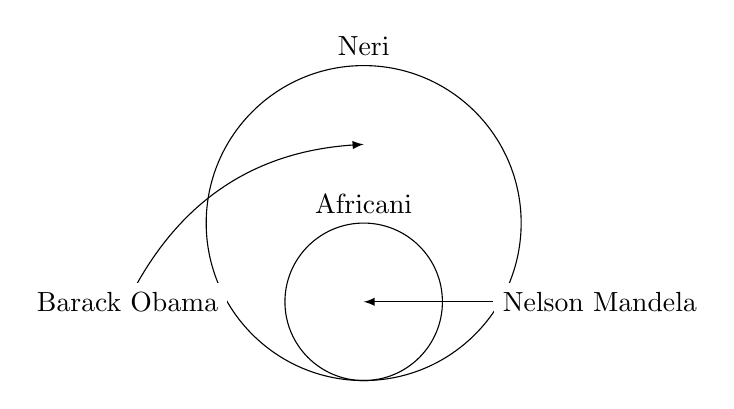
\begin{tikzpicture}
		\draw (0,0)circle[radius=1]  {};
		\draw (0,1)circle[radius=2]  {};
		\node [anchor=south]at (0,1) {Africani};
		\node [anchor=south]at (0,3) {Neri};
		\draw [-latex, bend left](-3, 0)node[fill = white]{Barack Obama}to(0,2);
    \node [fill = white](r)at (3,0) {Nelson Mandela};
		\draw [-latex](r)--(0,0);
	\end{tikzpicture}
\end{center}
\textit{Non è vero che tutti i neri sono africani, ma è vero che tutti gli africani sono neri}

\section{Logica}
Possiamo ragionare e trarre conclusioni tramite un nuovo concetto: l'entailment. Di base, un'asserzione $ a $, è vera solo se trova un corrispettivo fatto in un dato modello, ossia $ I_L\left(a\right) \in M $. Questo è detto entailment:
\begin{definizione}{Entailment}
	Data un'asserzione $ a \in \mathcal{L}_a$ e un modello $ M $, si dice che
	\[
		M |=_{\mathcal{L_a}} a
	\]
	se $ I_{\mathcal{L}_a} \left(a\right) \in  M $.
	\vskip3mm
	In modo simile, data una teoria $ \mathcal{T} = \left\{a\right\} $, allora
	\[
		M |=_{\mathcal{L_a}}  \mathcal{T}
	\]
	se $ I_{\mathcal{L}_a} \left(a\right) \in  M $ per ogni $ a \in \mathcal{T} $
\end{definizione}
Di fatto se $ M |= a $, significa che $ a $ è un'asserzione \underline{vera}. Quindi dato un modello di mondo si può definirne una logica attorno tramite la relazione di entailment:
\begin{definizione}{Logica del mondo}
	La logica del mondo è data da:
	\[
		L_W = \left<W, |=_{L_a}\right>
	\]
\end{definizione}
\begin{definizione}{Logica}
	Data una logica del mondo $  L_W = \left<W, |=_{L_a}\right> $, si può costruire una \underline{logica} ampliando il linguaggio $ L_a $ con nuove asserzioni complesse:
	\[
		L_l = \left<W, |=_{L}\right>
	\]
	dove $ L_a \in L $
\end{definizione}
L'idea è quindi quella di partire da un linguaggio semplice contentente sole asserzioni ($ L_A $), aggiungere nuove informaizoni (creo $ L $, t.c. $ L_a \in  L $) e verifico correttezza informazioni tramite il ragionamento ($ |=_{L} $)
\vskip3mm
Per formalizzare il meccanismo di ragionamento, si usano gli agenti:
\begin{definizione}{Agente}
	Data una logica $ L_W \left<W, |=_{\mathcal{L}_a}\right> $, un agente è dato da
	\[
		A_{L_L} = \left<L_L, \operatorname{Tell}, \operatorname{Ask}\right>
	\]
\end{definizione}
\begin{definizione}{Tell}
	L'operatore tell è definito come segue:
	\begin{enumerate}
		\item \underline{$ \operatorname{TellW}\left(A_L, w\right) $}: adds a word and extends the interpretation function and the domain if needed
		\item \underline{$ \operatorname{TellA}\left(A_L, a\right) $}: adds an \textit{axiom}, decreasing the partiality of the given theory
	\end{enumerate}
\end{definizione}\label{Tell}
\begin{definizione}{Ask}
	L'operatore ask è definito come segue:
	\begin{enumerate}
		\item \underline{$ \operatorname{AskC}\left(A_L, T\right) $}: \textit{ask check}. Ritorna {\ttfamily true} se $ T |= M $
		\item \underline{$ \operatorname{AskS}\left(A_L, T\right) $}: \textit{ask satisfiability} Ritorna {\ttfamily true} se $ T $ è soddisfabile, ossia esiste un $ M $ tale per cui $ T |= M $
	\end{enumerate}
\end{definizione}\label{Ask}
\begin{definizione}{Operatori logici}
	Gli operatori ask(\ref{Ask}) e tell(\ref{Tell}) possono essere scritti anche come segue:
	\begin{enumerate}
		\item $ M {?=} T $ ossia $ \operatorname{AskC}\left(A, T\right) $ \textit{teoria è corretta}
		\item $ D {??=} T $ ossia $ \operatorname{AskS}\left(A, T\right) $ \textit{teoria è soddisfabile}
		\item $ D != A $ ossia $ \operatorname{TellL}\left(A, L\right) $ \textit{amplia il linguaggio}
		\item $ M != T $ ossia $ \operatorname{TellT}\left(A, T\right) $ \textit{amplia la teoria con assiami}
	\end{enumerate}
\end{definizione}

\newpage
\begin{center}
	\begin{tikzpicture}[node distance = 9em]
		\node (1)[] at (0,0) {$ a $};
		\node (2)[right of = 1] {$ \mathcal{T}a $};
		\node (3)[right of = 2] {$ \mathcal{L} a $};
		\node (4)[below of = 1] {$f$};
		\node (5)[right of = 4] {$M$};
		\node (6)[right of = 5] {$D$};

		\draw [-latex](2)--(1) node [midway, above] {$ \in $};
		\draw [-latex](5)--(4) node [midway, above] {$ \in $};

		\draw [-latex](2)--(3) node [midway, above] {$ \subset $};
		\draw [-latex](5)--(6) node [midway, above] {$ \subset $};

		\draw [-latex](1)--(4) node (ta1) [midway, left] {$ Ta $};
		\draw [latex-](2)--(5) node (ta2)[midway, left] {$ |=_{a} $};
		\draw [-latex](3)--(6) node (ta3)[midway, left] {$ I_a $};

		\node (e1)[fit = (2) (5) (ta2), draw, dashed]  {};
		\node [anchor = south, align = center] at (e1.north) {World\\ representation};
		\node (e2)[fit = (3) (6) (ta3), draw, dashed]  {};
		\node [anchor = south, align = center] at (e2.north)  {World\\ model};
	\end{tikzpicture}
\end{center}
\begin{itemize}
	\item $ I_a $: interpretaion function
	\item $ |=_{a} $: world entailmen
	\item \textit{World model} $ W = \left<\mathcal{L}a , D, I_a\right>$
	\item \textit{World representation} $ R = \left< \mathcal{T}a, M\right> $
	\item \textit{World logic} $ L_w = \left<W, |=_{La}\right> $
	\item \textit{Logic} $ L_L = \left<W, |=_{L}\right> $
\end{itemize}


\end{document}
